\chapter{Solution Design: Improved Kepler Visualisation Tool (IKVT)}\label{C:sd}
This section discusses the design of the deliverable visualisation, the Improved
Kepler Visualisation Tool (IKVT). It details
the key design decisions revolving around structure, aesthetics, and
functionality that were made about the visualisation. 
% Description of tool
This project aims to improve an existing visualisation, The Kepler Visualisation
Tool which was discussed in the previous chapter. Whist this existing
visualisation displays exoplanets and some of their features, it lacks
interactivity for users trying to use it to gain information contained in the
Kepler Exoplanet Database effectively. The IKVT expands on this pre-existing
visualisation by adding key elements of interactivity missing in the existing
 visualisation as well as further enhancing the range and amount of data that
is available to users about exoplanets. The IKVT also incorporates a novel
gesture based interactive mechanism to the visualisation using a Microsoft
Kinect Sensor.

\section{System design and structure}
Because this project builds upon an existing system, complete comprehension of
how it is designed and how it functions is important. Going ahead in the
creation of the visualisation without this knowledge would create opportunities
for mistakes and incorrect assumptions about how the visualisation needs to be
created. To solve this issue diagrams the Unified Modeling Language(UML) were
used. In UML there are two basic categories of diagrams: structure diagrams and
behavior diagrams. Every UML diagram belongs to one these two diagram
categories. The purpose of structure diagrams is to show the static structure of
the system being modeled ie class diagrams, and or object diagrams. Behavioral
diagrams, on the other hand, show the dynamic behavior between the objects in
the system, including things like their methods, collaborations, and activities
ie, use case, and sequence diagrams
http://www.ibm.com/developerworks/rational/library/content/RationalEdge/sep04/be
ll/. For this project sequence diagrams and and class diagrams were used to help
understand the exisiting system and plan out the extensions, these are discussed
next.

\begin{enumerate}
\clearpage
{\bf \item UML Sequence Diagram}
  A sequence diagram is a diagram that primarily shows the interactions between
objects in the sequential order that those interactions occur.
For this project it was used to understand how each of the objects in the system
worked together to create the visualisation. Without understanding which objects
were responsible for each part of the render cycle would have made it difficult
to extend the visualisation. Through the sequence diagram we can see when each
of the objects in the system are updated, and when they are rendered. 
   \begin{figure}[H]
  \centering
      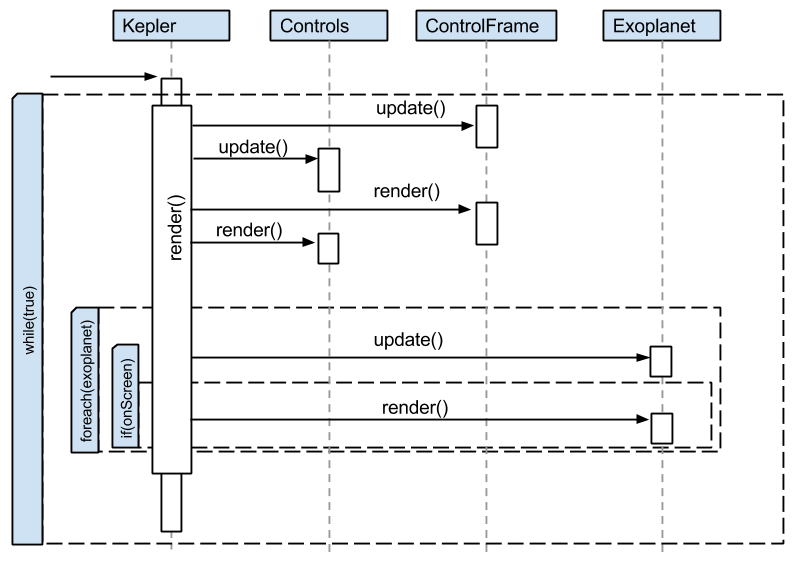
\includegraphics[width=0.8\textwidth]{images/sequence.png}
  \caption{Sequence Diagram of IKVT render cycle}  
    \label{fig:sequenceDiagram}
\end{figure}
\clearpage
 {\bf \item UML Class Diagram}
 Class diagrams describe the structure of a system by showing the system's
classes, their attributes, methods, and the relationships among objects.
 Developers can use class diagrams to design and document the system's coded (or
soon tbe coded) classes. For this project class diagrams were used to understand
the makeup of the existing KVT and then to plan the extensions. This class
diagram was maintained with the improvements introduced in the the visualisation
to provide an overview that could be used for further planning.
 \begin{figure}[H]
  \centering
      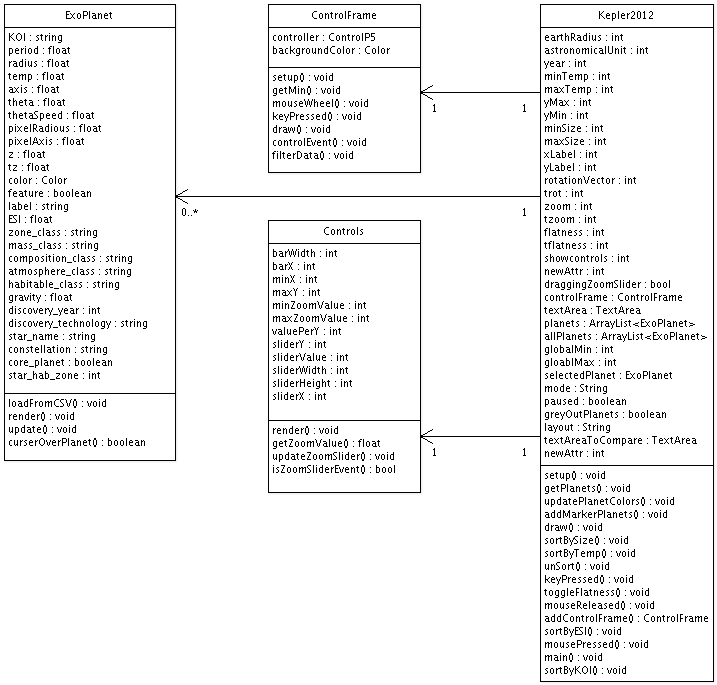
\includegraphics[width=0.8\textwidth]{images/classDiagram.png}
  \caption{Class Diagram of IKVT}  
  \label{fig:classDiagram}
\end{figure}
\end{enumerate}

By using
the sequence diagram in Figure \ref{fig:sequenceDiagram} coupled with the class
diagram in Figure\ref{fig:classDiagram} you can see where each method and field
is located and modified. This is a powerfull way of begining to understand an
exisitng system and then planning extensions.

\section{Visualisation Design}
The requirements produced in Chapter \ref{Chap:ra}: Requriements Analysis
provide a
description of the functionality that needs to be designed for this
visualisation. By adding additional details to these requirements we can specify
how the visualisation should look, behave, and function.

% By using abstract user interface design the layout and configuration of each
% element can be
% planned and coordinated without the need for excessive details which are
likely
% to change
% throughout the course of the project (e.g. colours and content) \cite{martin}.
\clearpage
\subsection{Functional Requirements}
\begin{enumerate}

{\bf
 \item[R1.] The visualisation needs to display planetary information to convey
knowledge to users.
}

  This requirement needs some form of textual display in order to convey enough
of the information about exoplanets to the user. This can be done with a Java
TextArea object to display each of the key
attributes of each Exoplanet. The following figure is a mockup of the text area
showing the information about each planet that would be displayed and the method
calls that would be used.

\begin{figure}[H]
  \centering
      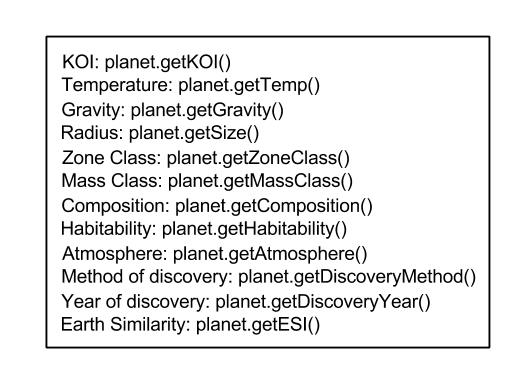
\includegraphics[width=0.8\textwidth]{images/textAreaMockup.png}
  \caption{Mockup of the TextArea}  
\end{figure}

To populate this text area it needs to be possible to select exoplanets, which
is discussed in the next requirement.
\clearpage
{\bf
 \item[R2.] The visualisation needs to allow exoplanets to be compared against
one another.}

There are two steps to fullfilling this requirement\\ 1. Allow selection of
exoplanets \\ 2. Display additional information about exoplanets when they are
selected.

The selection of exoplanets involves detecting when a user clicks and then
finding whether any planets are
located in that space. This is more complex in this system as it requires
detecting if the 3D space of each planet coincides with the 2D
location of the mouse click. When a planet is successfully selected it needs to
provide feedback and
information to the user to inform them that it has been selected and also to
provide relevant information.

\begin{figure}[H]
  \centering
      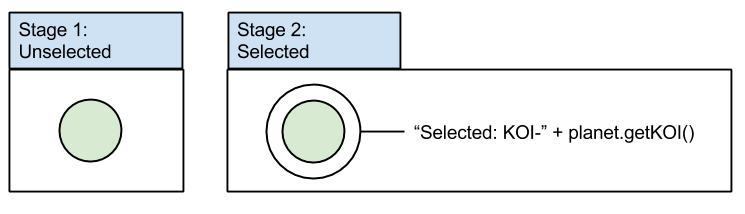
\includegraphics[width=.8\textwidth]{images/mockSelected.png}
  \caption{Mockup selection process}  
\end{figure}

In addition to this, when a planet has been successfully selected all of the
other planets in the
same solar system (sister planets) need to become highlighted. This can be done
by treating them as if they were selected and providing an additional indication
 to the user why they were highlighted.  
\begin{figure}[H]
  \centering
      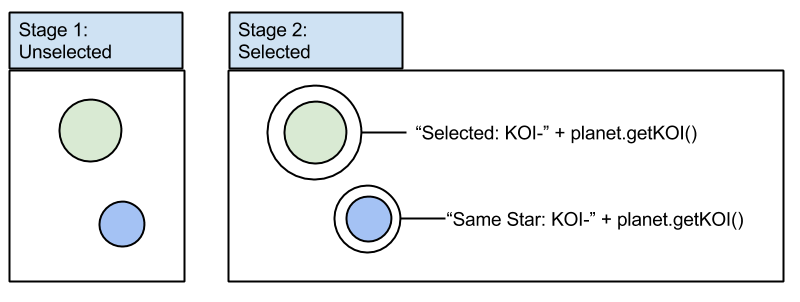
\includegraphics[width=.8\textwidth]{images/selectedSisterPlanets.png}
  \caption{Mockup highlight sister planets process}  
\end{figure}

There needs to be an efficient way that users can make comparisons between the
detailed textal information about exoplanets. By providing an additional text
box and allowing users to select multiple planets this can be accomplished.

\begin{figure}[H]
  \centering
      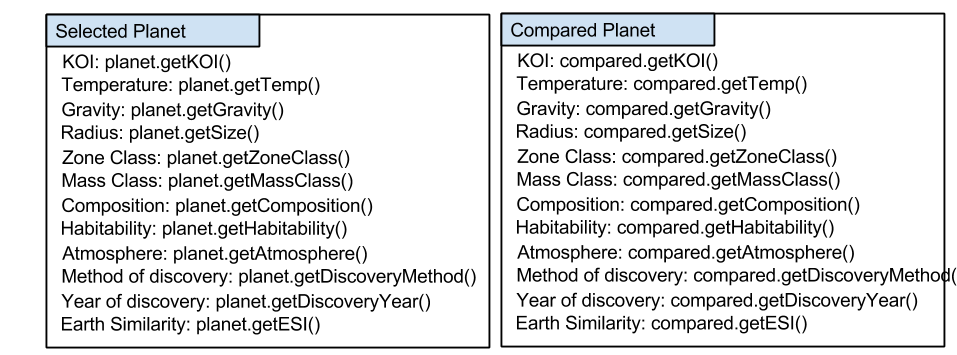
\includegraphics[width=.7\textwidth]{images/mockComparePlanets.png}
  \caption{Mockup compare planets text areas}  
\end{figure}
\clearpage

{\bf
 \item[R3.] The planets need to be able to be ordered by their similarity to
earth (ESI) and by their Kepler Object of Interest number (KOI).}

To fulfill this requirement the visualisation needs to allow users to view the
exoplanets in a way that uses the Earth as a point of reference and their Earth
Similarity Index (ESI) to order them and control their position. The following
figures display an abstract mockup of how this would be done.

\begin{figure}[H]
  \centering
      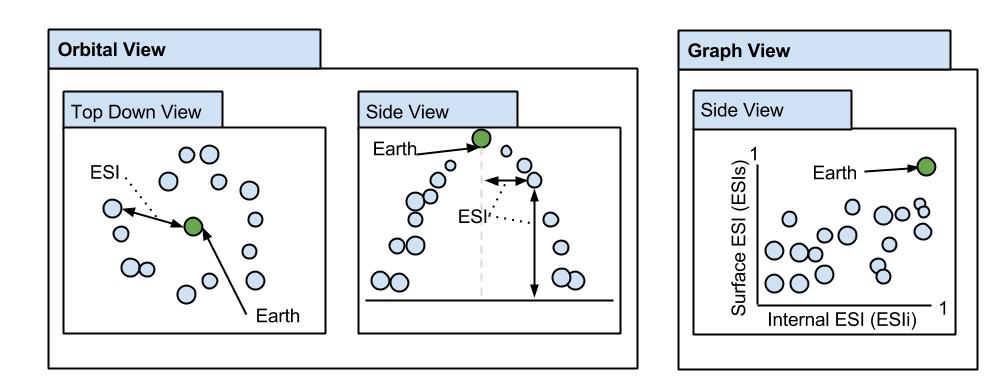
\includegraphics[width=1\textwidth]{images/mockupESI.png}
  \caption{Mockup of ESI views}  
\end{figure}

\clearpage
{\bf
 \item[R4.] The visualisation needs to allow users to define ranges of planetary
attributes to filter which planets are displayed.}

To fulfill this requirement a method of filtering exoplanets by their attributes
in order to control the number and types of planets displayed to the user. A
common method of achieving this is to use a set of sliders that allow a user to
filter something by a set of values. For example in this system a slider could
be used to control the size of planets that are displayed.

\begin{figure}[H]
  \centering
      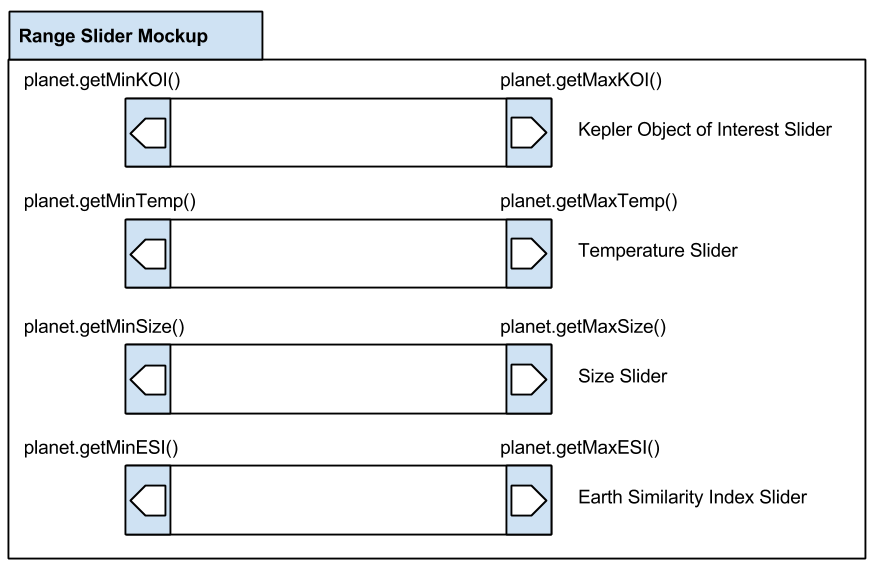
\includegraphics[width=.8\textwidth]{images/mockSlider.png}
  \caption{Mockup of range sliders}  
\end{figure}

In addition to this users should be able to easily sort the exoplanets to make
the most of the filtering. By allowing users to display the exoplanets sorted
vertically by the same attribute as the filters, they can easily see how
changing the filters affects the exoplanets displayed

\begin{figure}[H]
  \centering
      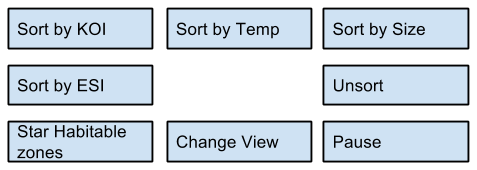
\includegraphics[width=0.5\textwidth]{images/mockButtons.png}
  \caption{Mockup of interactive buttons}  
\end{figure}

\clearpage
{\bf
 \item[R5.] Users need to be able to view the habitable zones of stars in
relation to the planets orbiting them.}

To display the habitable zones of the stars of each exoplanet a way to display
the hot (to close to the star), cold (to far from the star), and the habitable
zone (in between hot and cold zones) is required. This can be done by showing
the selected exoplanet in relation to its star by means of coloured circles
depicting where the exoplanet sits inside the zones, as displayed in Figure
\ref{fig:hab}. 

\begin{figure}[H]
  \centering
      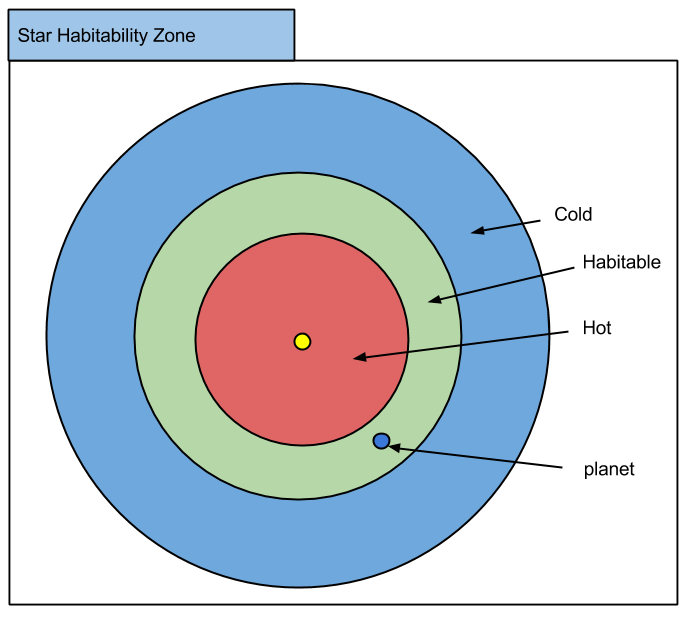
\includegraphics[width=.5\textwidth]{images/mockStarHabitability.png}
  \caption{Mockup star habitability zone}  
  \label{fig:hab}
\end{figure}




\end{enumerate}
\clearpage
\subsection{Nonfunctional Requirement}

\begin{enumerate}


{\bf \item[R6.] All interaction methods must be visible and intuitive.}

To make an interactive visualisation useable the controlls and interactive
methods need to be clear to users. To achieve this for IKVT an interactive panel
should be introduced. This panel should contain all of the interactive elements
of the visualisation in a single central place that is spacially seperated from
the main visualisation. This spacial seperation is imporatant as it reduces
cognitive load on users by allowing them to focus on the visualisation iteslef
until they need to use the panel in which case they can focus on that. It also
means that users only need to look in one place for all of the interactive
elements which reduces the risk of confusion. In this visualisation this
interactive panel would contain all of the interactive elements as discussed in
the previous requirements as displayed below in Figure
\ref{fig:interactionPanelMock}.

\begin{figure}[H]
  \centering
      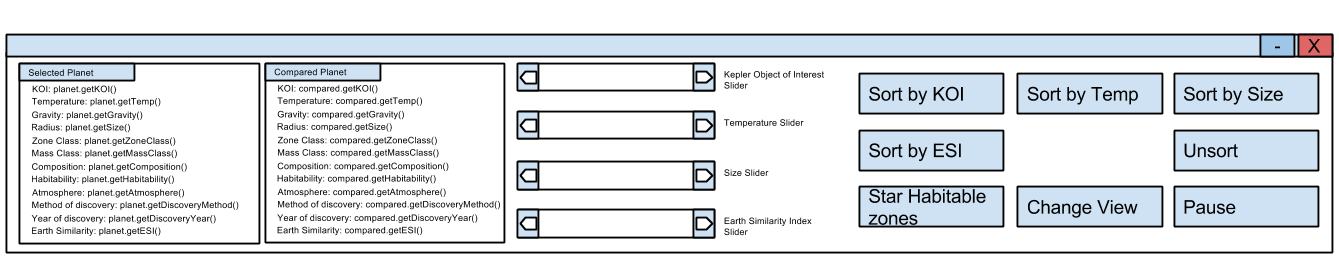
\includegraphics[width=1\textwidth]{images/allTogether.png}
  \caption{Mockup of the interaction panel}  
  \label{fig:interactionPanelMock}
\end{figure}

\clearpage
{\bf \item[R7.] The visualisation must remain uncluttered.}

The visualisation must not show so much information that it
causes information overload for users. The ability to filter and sort the
exoplanets gives a user the tools needed to
reduce the quantity of planets displayed in the visualisation and thus the
information load imposed on users. In addition to this, by having the text area
that displays the information about
selected planets separate from the main visualisation it reduces the cognitive
load on users as they don't have to use this component until they want to. ...~

\clearpage
{\bf  \item[R8.] There needs to be two modes of interaction with the system,
keyboard and mouse vs gesture based.}

The above requirements mostly relate to the keyboard an mouse system although
some of the requirements can carry over to a gesture based system. By
incorporating a novel interactive method using a Microsoft Kinect sensor it
gives users an alternative method of controlling the visualisation. For this to
be successfull it means incorporating a
means of detecting the gestures of users and linking them to an action in the
visualisation. A simple way to do this is to provide an area for the user to
gesture to on the screen that controls the movement of the camera in the
visualisation as shown in Figure \ref{fig:kinectMock}.
\begin{figure}[H]
  \centering
      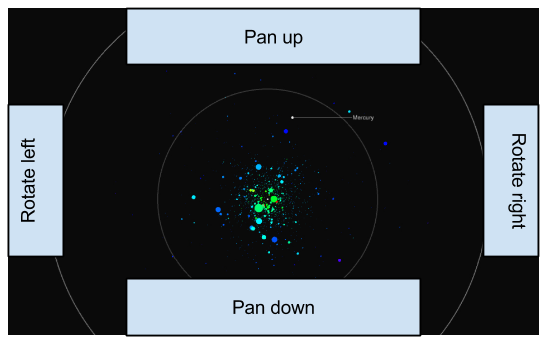
\includegraphics[width=0.7\textwidth]{images/mockKinect.png}
  \caption{Mockup of the Kinect system}
  \label{fig:kinectMock}
\end{figure}

In addition to controling the movement of the camera users need to be able to
zoom in and out of the visualisation as well as select exoplanets for further
examination as needed for the requirements. To do this a user should be able to
push and pull his/her hand from the screen to zoom in and out, as well as
gesturing to a planet to make a selection.

As the Kinect sensor no longer requires the use of a mouse the visualisation
design needs to be modified to accommodate the use of gestures. This meant
incorporating new cursors to indicate the state of the visualisation.
There are 7 states that the cursor needs to be able to be in to inform the user
of what action they are performing. These states are

\begin{enumerate}
 \item default cursor, hand is at rest
 \item panning up, hand is raised
 \item panning down, hand is lowered
 \item rotating left, hand is to the left
 \item rotating right, hand is to the right
 \item zooming in, hand is pressed forward
 \item zooming out, hand is pulled backwards
\end{enumerate}
Having a range of icons that clearly display these states is vital for keeping
the user informed of what they are doing. The proposed icons for this are
displayed below in Figure \ref{fig:cursors}
\begin{figure}[H]
  \centering
      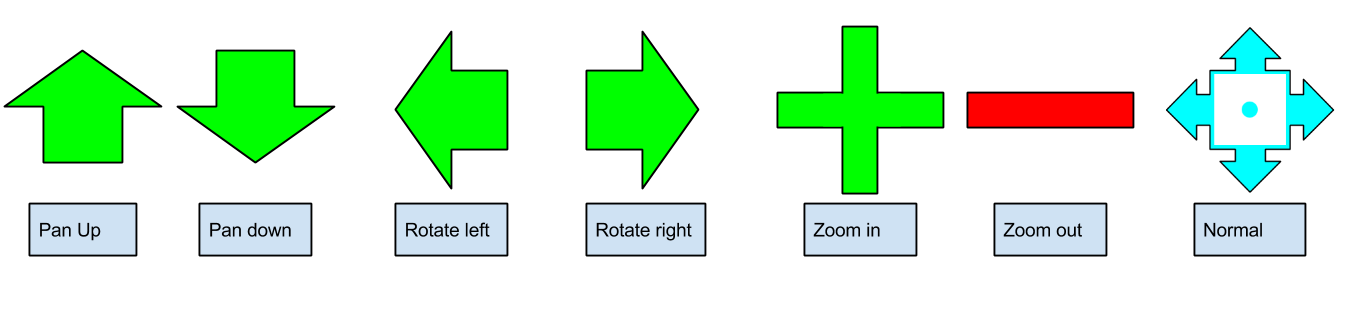
\includegraphics[width=0.9\textwidth]{images/curserImages.png}
  \caption{Mockup of cursor images for Kinect system}  
  \label{fig:cursors}
\end{figure}

No gesture design has been included for interacting wiht the interaction panel.
This is because the Microsoft Kinect sensor implementation in this visualisation
is intended as a proof of concept that interaction via gestures can allow users
to access the information within the system. If the user study discussed in
Chapter \ref{C:eval}: Visualisation Evaluation shows that gesture interaction is
successfull in this regard then incorporating it further can be undertaken.
\end{enumerate}

These solution designs were used for the implementation of IKVT which is discussed in the next chapter, Chapter \ref{C:sd}.
